\documentclass[11pt]{beamer}



\usepackage[utf8]{inputenc} %unix-windows-compatible
\usepackage{german}
\usepackage{fancyhdr} % Required for custom headers
\usepackage{lastpage} % Required to determine the last page for the footer
\usepackage{extramarks} % Required for headers and footers
%\usepackage[usenames,dvipsnames]{color} % Required for custom colors
\usepackage{graphicx} % Required to insert images
\usepackage{listings} % Required for insertion of code
\usepackage[section]{placeins}
\usepackage{caption} % to set figure captions in minipage
\usepackage{amsmath}
\usepackage{amssymb}
\usepackage{tikz}
\usetikzlibrary{matrix,chains,scopes,positioning,arrows,fit}
\usepackage{commath}
\usepackage{kpfonts}
\usepackage{algorithm}
\newcommand{\pushcode}[1][1]{\hskip\dimexpr#1\algorithmicindent\relax}
\usepackage[noend]{algpseudocode}

\usepackage{tcolorbox}
\usepackage{lipsum}

% (captionof{figure}{..}) Margins
%\topmargin=-0.45in
%\evensidemargin=0in
%\oddsidemargin=0in
%\textwidth=6.5in
%\textheight=9.0in
%\headsep=0.25in

%\linespread{1.1} % Line spacing
% tikz visibility on frames
\tikzset{
	invisible/.style={opacity=0},
	visible on/.style={alt={#1{}{invisible}}},
	alt/.code args={<#1>#2#3}{%
		\alt<#1>{\pgfkeysalso{#2}}{\pgfkeysalso{#3}} % \pgfkeysalso doesn't change the path
	},
}
% Set up the header and footer



\newtheorem{mydef}{Definition}
\newtheorem{theo}{Theorem}
\newtheorem{cor}{Corollary}


\makeatother
\setbeamertemplate{footline}
{
	\leavevmode%
	\hbox{%
		\begin{beamercolorbox}[wd=.4\paperwidth,ht=2.25ex,dp=1ex,center]{author in head/foot}%
			\usebeamerfont{author in head/foot}\insertshortauthor
		\end{beamercolorbox}%
		\begin{beamercolorbox}[wd=.6\paperwidth,ht=2.25ex,dp=1ex,center]{title in head/foot}%
			\usebeamerfont{title in head/foot}\insertshorttitle\hspace*{3em}
			\insertframenumber{} / \inserttotalframenumber\hspace*{1ex}
		\end{beamercolorbox}}%
		\vskip0pt%
	}
	\makeatletter
	\setbeamertemplate{navigation symbols}{}

\AtBeginSection[]
{
	\begin{frame}[plain]
		\frametitle{Table of Contents}
		\tableofcontents[currentsection]
	\end{frame}
}


\begin{document}


	\title %optional
	{Enhanced exact algorithms for discrete bilevel linear problems}
	\subtitle{Seminar: Computing Optimal Steiner Trees in Graphs}
	
	\author % (optional, for multiple authors)
	{Leon Eifler}
	
	\institute % (optional)
	{
	
		Institut f"ur Mathematik\\
		Technische Universit"at Berlin
		
	}
	
	\date % (optional)
	{01.07.2016}
	

	\begin{frame}
	\titlepage

	\end{frame}
	
\begin{frame}
	\frametitle{Table of Contents}
	\tableofcontents
\end{frame}

\section{Introduction}

\begin{frame} 
	\frametitle{Overview}
	\begin{itemize}
		\item Is a factor-2 approximation algorithm for the Prize-Collecting Steiner Tree Problem (PCST)
		\item Runs in $\mathcal O(d m \log n)$
		\item Builds solution by recursively merging clusters
		\item Uses dynamic edge-splitting to do this
	\end{itemize}
\end{frame}

\begin{frame} 
	\frametitle{The PCST}
	\begin{itemize}
		\item Given an undirected, connected graph $G=(V,E)$ with edge weights $c:E \rightarrow \mathbb{R}^+_0$ and node prizes $\pi :V \to \mathbb{R}^+_0$. 
			\begin{tcolorbox}[colback=green!5,colframe=green!40!black,title=PCST]
				Find a subtree $T$ of $G$, such that $c(T)+\pi(\bar T)$ is minimized
			\end{tcolorbox}
	\end{itemize}
\end{frame}

\begin{frame} 
	\frametitle{Laminar Family}
	\begin{mydef}[Laminar family.]
		A family $\mathcal{L}$ of non-empty subsets of $V$ is a laminar family if one of the following three cases holds for all $L_1, L_2 \in \mathcal{L}$:
		\begin{align*}
		(i) \ L_1 \cap L_2 = \emptyset && (ii) \ L_1 \subseteq L_2 && (iii) \ L_2 \subseteq L_1
		\end{align*}
	\end{mydef}
\end{frame}

\section{The original algorithm}
\begin{frame} 
	\frametitle{The Goemans-Williamson (GW) algorithm}
	\begin{itemize}
		\item Start with each node in its own singleton cluster. All clusters are active
		\item Merge and deactivate clusters until a single active cluster remains
		\item Maintain a spanning tree for each cluster 
		\item When finished, remove unnecessary nodes
	\end{itemize}
	\begin{theo}
			Both the original algorithm as well as the fast adaptive variant satisfy the
			approximation inequality
		\begin{equation*}
			c(T)+2\pi(\bar T) \le 2 c(T_{OPT}) + 2\pi (T_{OPT})
		\end{equation*}
	\end{theo}
\end{frame}

\begin{frame} 
	\frametitle{Moats}
		\begin{itemize}
	\item Maintain a $\textbf{moat}$ $y_C \in \mathbb{R}^+$, satisfying:
		
		\begin{tcolorbox}[colback=green!5,colframe=green!40!black,title=Edge-inequality]
			Let $\mathcal{C}$ be the set of clusters with one endnode of $e$ inside but not both. Then
			\begin{equation*}
			\sum_{C \in \mathcal{C}} y_C \le c(e).
			\end{equation*}
		\end{tcolorbox}
		\begin{tcolorbox}[colback=green!5,colframe=green!40!black,title=Cluster-inequality]
			For every cluster $C$, let $C'$ be the set with $C' \subseteq C$. Then
			\begin{equation*}
			\sum_{C' \in \mathcal{C}}y_{C'} \le \sum_{v \in C} \pi(v).
			\end{equation*}
		\end{tcolorbox}
		\item Moats are dual variables of a LP-relaxation 
	\end{itemize}
\end{frame}

\begin{frame}
	\frametitle{Primal-Dual Interpretation}
	\textbf{Primal LP}
	\begin{align*}
		\min \sum_{e \in E} c_e x_e + \sum_{i \in V} (1-s_i) \pi_i& \\
		 s.th. \quad x(\delta(S)) &\ge s_i && \forall i \in S, S \subseteq V \\
		s_i, x_e&\ge 0 && \forall i \in V, \forall e \in E
	\end{align*}
	
	\textbf{Dual LP}
	\begin{align*}
		\max \sum_{C  \subseteq V} y_S & \\
		s.th. \quad \sum_{C: e \in \delta(C)} y_C &\le c_e && \forall e \in E \\
		\sum_{C'  \subseteq C}y_{C'} &\le \sum_{v \in C} \pi(v) && \forall C  \subseteq V \\
		y_C &\ge 0 && \forall C \subseteq V
	\end{align*}
\end{frame}

\begin{frame}[shrink=10, plain]
	\begin{algorithm}[H]
		\caption{ The original GW-algorithm }\label{euclid}
		\begin{algorithmic}[1]
			\Function{GW-Algorithm}{$V,E,c,\pi$}
			\State Initialize a singleton active cluster for each node. Set all moat-values 0.
			\State Initialize the spanning forest $F$.
			\While{At least one cluster is active}
			\State Increase the moat values $y_C$ on all active Clusters $C$ until  a constraint (edge or cluster) becomes tight.
			\If{ edge constraint becomes tight for $e = (u,v)$}
			\State Let $C_u, C_v \in \mathcal{L}$ be the maximal clusters
			\State Deactivate $C_u$ and $C_v$.
			\State Create $C' = C_u \cup C_v$ as active cluster in $\mathcal{L}$.
			\State Set the moat $y_{C'} = 0$.
			\State Remove all $e'$ with both endpoints in $C'$ from $E$.
			\State Add $e$ to $F$.
			\EndIf
			\If{ cluster constraints becomes tight for $C$ }
			\State Deactivate $C$
			\EndIf
			\EndWhile
			\State Prune F of unnecessary nodes 
			\EndFunction
		\end{algorithmic}
	\end{algorithm}
\end{frame}

\begin{frame} 
	\frametitle{Properties}
	\begin{itemize}
		\item The while loop is called at most $2n$ times.
		\item Can be difficult to determine which constraint becomes tight next
		\item Clusters can be deactivated and reactivated several times \\
		  $\rightarrow \mathcal{O}(n\log n)$
		\item Overall runtime: $\mathcal{O}(n^2 \log n)$.
	\end{itemize}
\end{frame}
\begin{frame} 
	\frametitle{Example}
	\center
	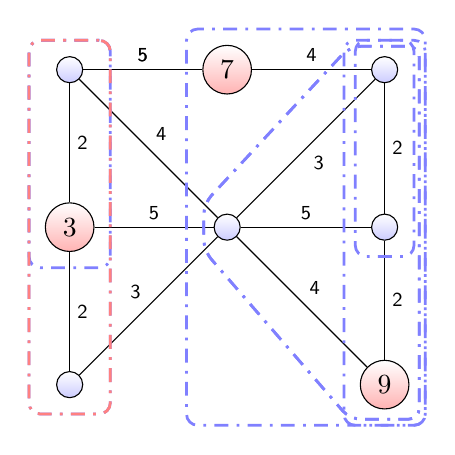
\begin{tikzpicture}[
	node/.style = {shape=circle, rounded corners, node distance=2cm,
		draw, align=center,
		top color=white, bottom color=blue!20},
	terminal/.style     = {node, bottom color=red!30},
	normal/.style      = {node, font=\ttfamily\normalsize}]

	\node[normal](1){};
	\node[right  of = 1, terminal](2){7};
	\node[below  of = 1, terminal](3){3};
	\node[right  of = 2, normal](4){};
	\node[right  of = 3, normal](5){};
	\node[below  of = 3, normal](6){};
	\node[below  of = 4, normal](7){};
	\node[below  of = 7, terminal](8){9};
	
	\path[every node/.style={font=\sffamily\small,scale=.8}]  
	(1) edge node [left,auto] {5}(2)
	(2) edge node [left,auto] {4}(4)
	(1) edge node [left,auto] {2}(3)
	(1) edge node [left,auto] {5}(2)
	(4) edge node [left,auto] {2}(7)
	(3) edge node [left,auto] {5}(5)
	(5) edge node [left,auto] {5}(7)
	(1) edge node [left,auto] {4}(5)
	(4) edge node [left,auto] {3}(5)
	(3) edge node [left,auto] {2}(6)
	(7) edge node [left,auto] {2}(8)
	(6) edge node [left,auto] {3}(5)
	(5) edge node [left,auto] {4}(8);
	
	
	\tikzset{blue dotted/.style={draw=blue!50!white, line width=1pt,
			dash pattern=on 1pt off 3pt on 5pt off 3pt,
			inner sep=2mm, rectangle, rounded corners}};
		\tikzset{red dotted/.style={draw=red!50!white, line width=1pt,
				dash pattern=on 1pt off 3pt on 5pt off 3pt,
				inner sep=2mm, rectangle, rounded corners}};
		
	
	% Finally the blue dotted boxes are drawn as nodes fitted to other nodes
	\node (first dotted box) [blue dotted, visible on=<2>,
	fit = (1)(3) ] {};
	\node (first dotted box) [blue dotted, visible on=<3>,
	fit = (1)(3)(6) ] {};
	fit = (1)(3) ] {};
	\node (first dotted box) [red dotted, visible on=<4->,
	fit = (1)(3)(6) ] {};
	\node (first dotted box) [blue dotted, visible on=<5>,
	fit = (4)(7) ] {};
	\node (first dotted box) [blue dotted, visible on=<6>,
	fit = (4)(7)(8) ] {};
	
	\node[fit=(4) (7) (8)] (n12) {};
	\node[fit=(5) (7)] (n23) {};
	
	\draw[blue dotted, visible on = <7>] (n23.north west) -- (n12.north west) 
	-- (n12.north east) -- (n12.south east) -- (n12.south west) --(n23.south west) -- cycle;
	
	\draw[blue dotted, visible on = <7>] (n23.north west) -- (n12.north west) 
	-- (n12.north east) -- (n12.south east) -- (n12.south west) --(n23.south west) -- cycle;
	
	\node (first dotted box) [blue dotted, visible on=<8>,
	fit = (4)(7)(8)(5)(2) ] {};
	
	\end{tikzpicture}
\end{frame}

\section{The fast variant}

\begin{frame} 
	\frametitle{High-level description}
	\begin{itemize}
		\item Produces exactly the same result as original scheme
		\item Split every edge $e=(u,v)$ into two parts $e_u, e_v$.
		\item Use \textbf{events} to quickly determine which edge has to be considered next
	\end{itemize}
\end{frame}

\begin{frame} 
	\frametitle{Preliminaries}
	\begin{description}
		\item[event-value $\mu(p)$] Amount of time until edge-event occurs. For each $e=(u,v)$, we have $\mu(e_u)+\mu(e_v) = c_e$.
		\item[slack] The remaining slack of an edge part is	$\mu(e_u) - \sum_{C \in \mathcal{C}} y_C$
		\item[Data structures] \ \\
		\begin{itemize}
			\item Priority Queue $Q_C$ for each Cluster, managing edge-events
			\item Overall Priority queue of all the queues \\
			$\rightarrow$ Heap of heaps
			\item Priority Queue of Cluster-events
		\end{itemize}
	\end{description}
\end{frame}

\begin{frame}[plain, shrink=30]
	\begin{algorithm}[H]
		\caption{ Fast variant of the GW-scheme }
		\begin{algorithmic}[1]
			\Function{PCSTFast}{$V,E,c,\pi$}
			\State Initialize (data-structures, cluster, forest)
			\State $t \leftarrow 0$ \Comment{Current time}
			\State $\alpha \leftarrow n$ \Comment{Number of active clusters}
			\While{$\alpha > 1$}
			\State $(t_e,p_u) \leftarrow$ \Call{GetNextEdgeEvent}{\null}
			\State $(t_C,C) \leftarrow$ \Call{GetNextClusterEvent}{\null}
			\If{ $t_e < t_c$}
			\State $t \leftarrow t_e$
			\State \Call{RemoveNextEdgeEvent}{\null} 
			\State $p_v \leftarrow$ \Call{GetOtherEdgePart}{\null}
			\State $(s,C_u) \leftarrow$ \Call{GetSumOnEdgePart}{$p_u$}
			\State $(s',C_v) \leftarrow$ \Call{GetSumOnEdgePart}{$p_v$}
			\State $r \leftarrow c(u,v) - s - s'$ \Comment{Remaining slack}
			\If{ $C_u = C_v$} \Comment{Edge completely in one cluster}
			\State continue
			\EndIf
			\If{ $r = 0$}
			\State \Call{MergeClusters}{$C_u,C_v$}
			\Else
			\State \Call{GenerateNewEdgeEvents}{$p_u,p_v$}
			\EndIf
			\Else
			\State $t \leftarrow t_c$
			\State \Call{RemoveNextClusterEvent}{\null}
			\State \Call{DeactivateCluster}{$C$}
			\State $\alpha \leftarrow \alpha -1$
			\EndIf
			\EndWhile
			\State \Call{PruneTree}{\null}
			\EndFunction
		\end{algorithmic}
	\end{algorithm}
\end{frame}

\begin{frame} 
	\frametitle{\textproc{MergeClusters($C_u,C_v$)}}
	\begin{itemize}
		\item Mark both inactive and remove from Queues
		\item If $C_u$ is inactive since time $t'$, increase the keys of all events in $Q_{C_u}$ by $t-t'$
		\item Merge the queues and insert into heap of heaps
	\end{itemize}
\end{frame}

\begin{frame} 
	\frametitle{\textproc{GenerateNewEdgeEvents}($p_u,p_v$)}
	\begin{itemize}
		\item Invoked when edge event occurs but edge-constraint is not tight.
		\item If the cluster containg $v$ is active, split the remaining slack on both edge-parts
		\item Otherwise put all the slack on the event for $p_u$
	\end{itemize}
\end{frame}
\section{Analysis}

\begin{frame} 
	\frametitle{Running Time}
	\begin{theo}
		Let all node prizes $\pi(v)$ and all edge costs $c(e)$ be even integers. Then all cluster merge and deactivation events occur at integer times.
		\end{theo}
		\pause
		\begin{proof}
			\begin{itemize}
				\item By induction on possible time steps.
				\item Induction Hypothesis: Let $t_e$ be the time the edge-constraint for $e$ becomes tight, $t_C$ the time the cluster-constraint for $C$ becomes tight. Then both are integers. If we merge at time $t_e$ between an active and inactive cluster, then $t_e-t_{inactive(C)}$ is even.
				\item Case analysis over possible events.
			\end{itemize}
		\end{proof}
	\end{frame}
	\begin{frame} 
		\frametitle{Running Time II}
		\begin{cor}
			Let all node prizes $\pi(v)$ and al edge costs $c(e)$ be specified with d bits of precision. Then the number of edge-part events is bounded by $\mathcal{O}(dm)$.
		\end{cor}
			\begin{theo}
				All subroutines in the algorithm can be implemented in $\mathcal{O}(\log n)$.
			\end{theo}
\end{frame}

    \begin{frame} 
    	\centering{\textbf{\Large{Thank you for your attention!}}}
    	\nocite{HegdeIndykSchmidt2014}
    	\nocite{Goemans:1992:GAT:139404.139468}
    	\bibliographystyle{abbrv}
    	\bibliography{Bibliography}
    \end{frame}

\end{document}
